\chapter{Introduzione}

\section{Sistemi dinamici}
Sono un'evoluzione temporale di un ingresso e un'uscita, vengono modellati dalle \textbf{equazioni differenziali}.\\
Vedremo sono funzioni monodimensionali (cioè dipendenti solo dal tempo) ma in realtà possiamo benissimo avere più dimensioni.\\
I modelli ci danno una stima del comportamento di una sistema, in particolare il modello delle equazioni differenziali si può svolgere: nel tempo, nel dominio della trasformata di Laplace (utile con i segnali esponenziali e sinusoidali) e nel dominio della trasformata di Fourier (è un restrizione di Laplace, è utile nei segnali sinusoidali).\\
Studieremo le proprietà dei sistemi, di queste la più importante è la stabilità.\\

\section{Modellare un sistema}
Modelliamo un sistema come fosse una scatola nera, avrà un segnale come input e output (es. suono 1D, immagine 2D).\\
I sistemi ci servono per vari motivi: possono facilitare la trasmissione di un segnale, migliorarlo accentuando alcune informazioni o eliminandone altre (filtraggio).\\
Vogliamo vedere i sistemi come \textbf{funzioni matematiche} (pag. 69 libro "Structure and Interpretation of Signals and Systems")\\

\begin{figure}
	\centering
	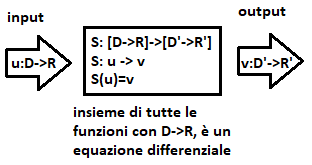
\includegraphics[width=0.7\linewidth]{immagini/sistema}
	\caption{ modello di un sistema come scatola nera}
	\label{fig:sistema}
\end{figure}



$ \forall s \in D' $ allora $ v(s)=(S(u))(s)\in R'  $ \\

\pagebreak

Abbiamo tre tipi di sistemi:\\
- Continui: operano su segnali continui\\
- Discreti: operano su segnali discreti\\
- Ibridi fra continui e discreti (non li vedremo)\\

\begin{figure}[h]
	\centering
	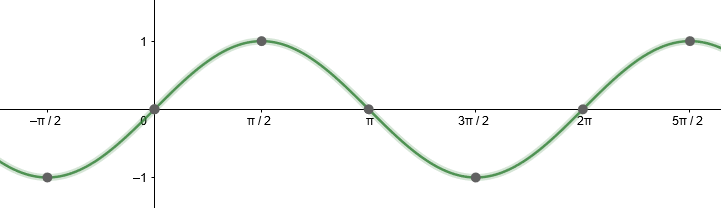
\includegraphics[width=0.7\linewidth]{immagini/seno}
	\caption{Segnale continuo}
	\label{fig:seno}
\end{figure}


\begin{figure}[h]
	\centering
	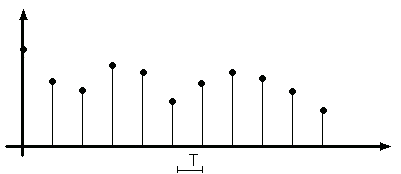
\includegraphics[width=0.7\linewidth]{immagini/tempo_discreto}
	\caption{ Segnale discreto}
	\label{fig:tempodiscreto}
\end{figure}

\section{Quantizzazione e campionamento}
Per andare da analogico a digitale (A->D) ho bisogno di campionamento e quantizzazione.\\

Campionamento: trasformiamo il dominio. Non ho sempre perdita di dati.\\

\begin{figure}[h]
	\centering
	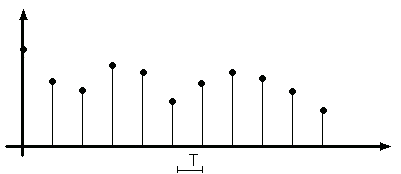
\includegraphics[width=0.7\linewidth]{immagini/tempo_discreto}
	\caption{ Segnale campionato nel tempo}
	\label{fig:tempodiscreto}
\end{figure}

\pagebreak
Quantizzazione: trasformiamo il codominio. Ha sempre perdita di informazione.\\

\begin{figure}[h]
	\centering
	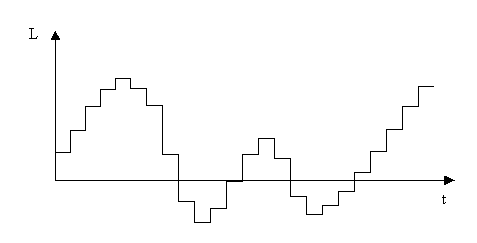
\includegraphics[width=0.7\linewidth]{immagini/quantizzato}
	\caption{ Segnale sinusoidale quantizzato nelle ampiezze}
	\label{fig:quantizzato}
\end{figure}

\section{Sistemi LTI}
Studiamo un tipo particolare di sistemi, che hanno due proprietà: linearità e tempo invarianza (L=lineari, TI=tempo invarianti).\\
- Linearità:\\
Se $ v_{1}=S(u_{1}) $ e $ v_{2}=S(u_{2})  $ 
allora $ S(\alpha u_{1} + \beta u_{2}) 
= \alpha S(u_{1}) + \beta S(u_{2})
= \alpha v_{1} + \beta v_{2} $ con $ \alpha , \beta \in C^{*} $ \\
Oppure grazie al \textbf{principio di sovrapposizione degli effetti} ( stabilisce che per un sistema dinamico lineare l'effetto di una somma di perturbazioni in ingresso è uguale alla somma degli effetti prodotti da ogni singola perturbazione): \\
$ S( \sum_{i=0}^n \alpha_i u_i ) 
=  \sum_{i=0}^n \alpha_i S( u_i )
$ \\
La linearità è dovuta alle equazioni differenziali, all'interno hanno la derivata prima che è essa stessa lineare.\\
- Tempo invariante:\\
 Significa che l'uscita non dipende esplicitamente dal tempo, cioè se un ingresso x(t) produce l'uscita y(t) allora per ogni ingresso traslato $x(t+ \delta )$ si ha un'uscita traslata dello stesso fattore $y(t+ \delta )$.\\
 
 $u(t+ t_0 ) \rightarrow v(t+ t_0 )$
 
\begin{figure}[h]
	\centering
	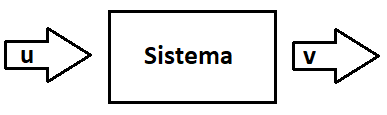
\includegraphics[width=0.7\linewidth]{immagini/sistema2}
	\caption{ Sistema generico }
	\label{fig:sistema2}
\end{figure}

\begin{figure}[h]
	\centering
	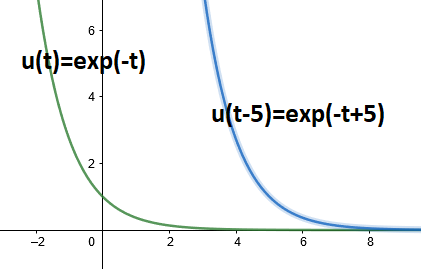
\includegraphics[width=0.7\linewidth]{immagini/esponenziale}
	\caption{ Esempio di tempo invariante }
	\label{fig:esponenziale}
\end{figure}

\pagebreak

I sistemi LTI che studieremo sono definiti da equazioni differenziali a coefficienti costanti.

Per i sistemi continui useremo il modello:
\begin{equation*}
\sum\limits_{i=0}^n a_{i} \frac{ d^{i} v }{ dt^{i}  } = \sum\limits_{i=0}^m b_{i} \frac{ d^{i} u }{ dt^{i}  }
\tag{1}\label{equation 1}
\end{equation*}
con $u$ e $v$ funzioni con dominio uguale a $\mathbb{R}$. In generale abbiamo $n\geq m$.


Per i sistemi discreti useremo il modello:
\begin{equation*}
\sum\limits_{i=0}^n a_{i} v(k-i) = \sum\limits_{i=0}^m b_{i} u(k-i)
\end{equation*}
con $u$ e $v$ funzioni con dominio uguale a $\mathbb{Z}$ e $ k \in \mathbb{Z} $.

\section{Sistemi SISO}
Per semplicità considereremo solo i sistemi SISO, cioè single input single output. Ma in generale i sistemi sono MIMO, cioè multiple input multiple output (questi non li vedremo).

\subsection*{Esempio semplice di un sistema}

Nel dominio del tempo rappresentiamo un sistema $S$ continuo come: \\
\begin{equation*}
S: [\mathbb{R} \rightarrow \mathbb{R}] \rightarrow [\mathbb{R} \rightarrow \mathbb{R}]
\end{equation*}

Abbiamo anche visto che modelliamo i sistemi con le derivate (che ehhh non ci piacciono molto) e vorremmo quindi qualcosa di più semplice. Usiamo Laplace (salvatore del popolo) che trasforma le derivate in moltiplicazioni ("Trasformò acqua in vino" semicit.). Le moltiplicazioni sono semplici e belle (insomma tanto love per le moltiplicazioni e per Laplace $\heartsuit$).\\

Nel dominio complesso o delle frequenze rappresentiamo quindi il sistema $S$ continuo come: \\
\begin{equation*}
S: [\mathbb{C} \rightarrow \mathbb{C}] \rightarrow [\mathbb{C} \rightarrow \mathbb{C}]
\end{equation*}

\begin{figure}[h]
	\centering
	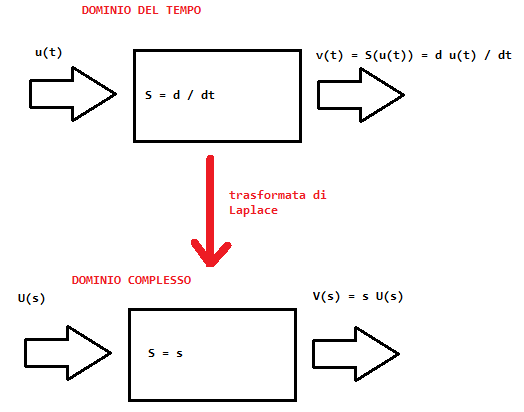
\includegraphics[width=0.7\linewidth]{immagini/LaplaceLove}
	\caption{ Come Laplace trasforma dal dominio del tempo a quello complesso }
	\label{fig: Sistema Laplace}
\end{figure}

\subsection*{Esempio di sistema discreto}
Consideriamo il sistema: \\
\begin{equation*}
	\begin{split}
	S: [\mathbb{Z} \rightarrow \mathbb{R}] \rightarrow [\mathbb{Z} \rightarrow \mathbb{R}] \\
	u \mapsto S(u) = v
	\end{split}
\end{equation*}
dove $v(n) = \dfrac{u(n)+u(n-1)}{2} \in \mathbb{R} $. Cioè l'output è $\forall n $ la media dell'input attuale e dell'input precedente (sistema moving average).\\
$u(n)$ può essere una qualsiasi funzione discreta. Prendiamo due esempi diversi di input.\\


Per primo esempio prendo come input:
\begin{equation*}
u(n)=
\begin{cases} 
	1, & \mbox{se }n\geq 0 \\ 
	0, & \mbox{altrimenti}
\end{cases} 
\end{equation*}

\begin{figure}[h]
	\centering
	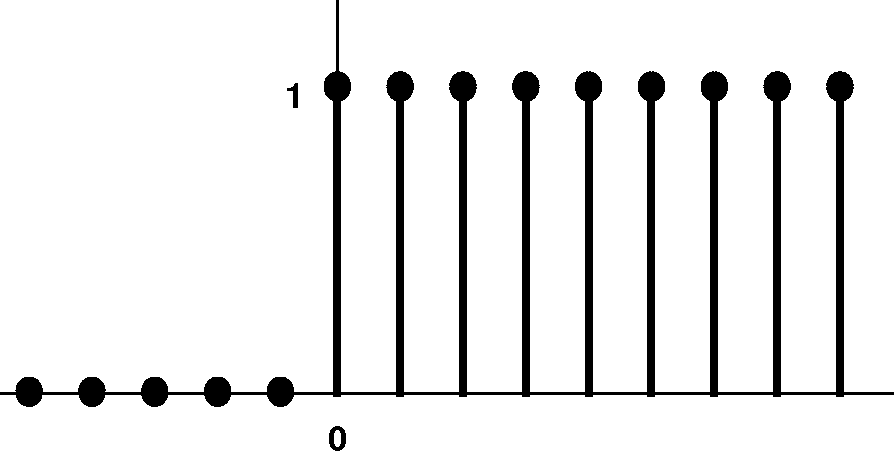
\includegraphics[scale=0.5]{immagini/gradino}
	\caption{ La funzione gradino (unit step) come input }
	\label{fig: Unit step}
\end{figure}

\pagebreak

Avrò come output:
\begin{equation*}
v(n)=
\begin{cases} 
0, & \mbox{se }n < 0 \\ 
1/2, & \mbox{se }n = 0 \\ 
1, & \mbox{se }n > 0
\end{cases} 
\end{equation*}

\begin{figure}[h]
	\centering
	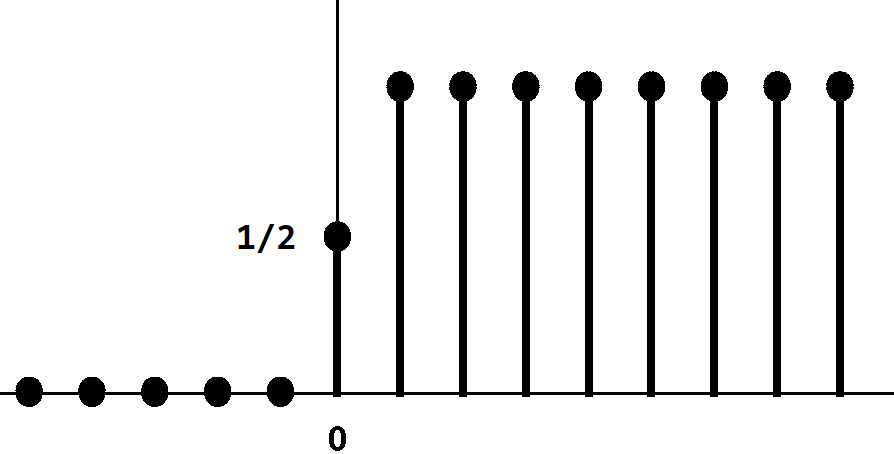
\includegraphics[scale=0.5]{immagini/gradinoMedia}
	\caption{ L'output del sistema moving average con in input la funzione gradino}
	\label{fig: Output sistema moving average gradino}
\end{figure}
Per secondo esempio prendo come input:
\begin{equation*}
u(n)= \cos(2\pi f n)
\end{equation*}
dove $n \in \mathbb{Z} $ e $f \in \mathbb{R}_{+}^{*}$\\
Avrò come output:
\begin{equation*}
v(n)= S(u)(n) = \frac{1}{2} (\cos(2\pi f n) + \cos(2\pi f (n-1))) = R\cos( 2\pi f n + \theta) \in \mathbb{R}^{*}
\end{equation*}
dove $\theta = \frac{1}{2} \arctan(\frac{ \sin (-2\pi f)    }{1+\cos(2\pi f)})$ e $ R = \sqrt{ 2+2\cos(2\pi f)} \in \mathbb{R}^{*}$\\
NB: Amplifico l'input sinudoidale con R ma il periodo e la frequenza rimangono invariate. In output quindi avrò ancora un segnale sinusoidale (questo fenomeno lo studieremo nella frequence responce).
